The implementation of the graphical user interface (GUI) required a number
of decisions to be made before writing it could begin, including of
course, how the team would be distributed between implementing the GUI
and the data models.

%---------------------------------------------------------------------

% Not the best place for this, but finding a better one will require
% restructuring during editing process.

\subsection{Programming Language}
\label{impl:ui:programminglanguage}

When discussing implementation, the group quickly settled on Java as
the language in which to implement the application, due to our 
collective experience with it as a consequence of the Java Programming
course taken in the previous academic year, and our knowledge of
existing GUI frameworks that would suit our purposes.

%---------------------------------------------------------------------

\subsection{GUI Framework}
\label{impl:ui:guiframework}

From a brief research period at the start of the implementation 
process, we settled on two possible options for a GUI framework to use
for the application. It's important to note that other GUI options are
available, but upon further analysis, it became clear that Swing and 
JavaFX were the most suitable to our needs.

%---------------------------------------------------------------------

\subsubsection{Swing}
\label{impl:ui:guiframework:swing}

Each member of the group had some limited experience with the Swing 
framework, though not all of it had been positive.
The experience each member of the team had with Swing varied, and
although every member had agreed that their experience had not been
entirely problem-free, we conceded that its integration with the Netbeans
Integrated Development Environment (IDE), discussed in section
\ref{impl:ui:ide:netbeans}, was extremely useful.

However, on investigating the framework more closely it was clear that
Swing was extremely well documented with full API specification
\cite{swingAPI}, and in-depth tutorials \cite{swingTutorial}.
This was a huge part of our decision as we felt that the documentation
provided would be more than adequate to allow us to use the framework
with relative comfort.

%---------------------------------------------------------------------

\subsubsection{JavaFX}
\label{impl:ui:guiframework:javafx}

Another framework considered was JavaFX which no member of the team
had any experience with. 
Some members felt that this was a risk worth taking, given how much
they disliked Swing, discussed above.
In reality JavaFX was only briefly considered and totally disregarded
when, upon brief investigation, JavaFX was still a relatively new
framework, and consequently, comprehensive documentation was not as
readily available for JavaFX as with Swing, particularly when it came 
to troubleshooting on online forums.

In addition, JavaFX required Java 7, which, again, no member of the
group had used before and which was not available, at the time, in the
Level 3 Laboratory where we would be working for the majority of the
year.
It seemed like too much of a risk to try to learn two different
technologies at the same time, while having to provide our own
development platforms, which, with various members of the team never
having used the Linux OS before, could potentially cause a number of
problems.

%---------------------------------------------------------------------

\subsubsection{Decision}
\label{impl:ui:guiframework:decision}

The investigation was carried out by the group's Toolsmith, Ross
Barnie, who presented the evidence discussed in the sections above
regarding the two frameworks to the rest of the team.
With this evidence the team voted in favor of using the Swing
framework with Java 6.

Retrospectively, Swing, and Java 6, are out-of-date technologies and
JavaFX is now packaged with Java 7 \cite{javafxOverview}, so the
application would have been more up-to-date or future-proof had we
used JavaFX.
Additionally, (some of) the computers in the level 3 lab now do have
Java 7 installed upon another project team requesting it, so our fears
over development platform problems were nullified, though this was
only after we had started development.

It was an unfortunate shortcoming of the research into JavaFX that the
group did not know about JavaFX's integration with the Netbeans IDE
which was seen as one of the key differences between the two
frameworks at the time of making the decision.

%---------------------------------------------------------------------
%---------------------------------------------------------------------

\subsection{IDE}
\label{impl:ui:ide}

One concern was that, in some members' experience, using two separate
IDEs was extremely time consuming, particularly while using version
control.
This was mostly due to various metadata that IDEs keep track of in
various files, however this meant that any small change to the source
code would change the metadata and therefore each commit would have to
involve adding it, which would be very time-consuming.

It is because of this experience that the group decided to work from a
single IDE, researched again by Ross Barnie.

%---------------------------------------------------------------------
\subsubsection{Netbeans}
\label{impl:ui:ide:netbeans}

Netbeans is an IDE which the team had had little experience with and had
only used in the context of building applications with GUIs created
using the Swing framework.
There was some trepidation to using Netbeans since most of the team
had associated their problems with Swing with Netbeans itself.
Upon further research, which involved using the IDE to build small
applications, Netbeans started much faster than Eclipse, discussed
below.
And the design interface was very simple and easy to use, with each
element being laid out the way you wish and the associated source code
being generated for you.
This meant that the design layout could be finished very quickly,
rather than spending our time writing hundreds of lines of source code
just for the interface.

In terms of Netbeans' metadata, it was quite minimal and would not
clutter the version control repository to an unacceptable degree.

%---------------------------------------------------------------------
\subsubsection{Eclipse}
\label{impl:ui:ide:eclipse}

The team had substantial knowledge of Eclipse from its mandated use in
Java Programming 2 \cite{javaProgramming2}. Again, our experience of 
Eclipse is somewhat tainted by associations with problems we faced at 
the time, such as a bug on the version for Windows which meant that 
Eclipse would freeze if you tried to copy or paste anything.

In our experience, we found Eclipse to be very slow, both during 
start-up and normal operation. 
Editing-wise, Eclipse was rather cumbersome and not much better than a
text editor.
Also the requirement to bind the ``Workspace'' was seen as a potential
point for confusion and errors.

In addition, the team felt that the missing design interface seen on
Netbeans, discussed above, was a huge disadvantage and would cause a
significant loss of time, simply due to the volume of code we would
have to write instead of being auto-generated.

Members of the team also pointed out that Eclipse has a tendency to
create a large amount of metadata which would clutter the version
control repository.

%---------------------------------------------------------------------
\subsubsection{No IDE}
\label{impl:ui:ide:noide}

It was briefly considered to have no IDE at all and simply use text
editors.
This would allow for extremely fast editing in a very comfortable
environment, since most text editors, such as Vim or Emacs, are highly
customisable and can launch in a matter of seconds.
Text editors would also not require metadata, keeping our version
controlled directories clean.

However, the obvious problem with no IDE is that troubleshooting
problems becomes very tedious very quickly, and unlike IDEs, you
cannot automatically import a missing package or method, nor can there
be any auto-generated code for that matter.

%---------------------------------------------------------------------
\subsubsection{Decision}
\label{impl:ui:ide:decision}

When the evidence above was given to the team, we were also discussing
which GUI Framework to use (as discussed in section
\ref{impl:ui:guiframework}) and it became obvious that integration
with the framework would be key to helping us develop the GUI.

We therefore decided to work with the Netbeans IDE because of the
design interface, minimal metadata, and lack of (known) bugs that
would affect us in any meaningful way.

Retrospectively, this was the correct decision.
Even if we had chosen a different GUI framework, the advantages of the
easy-to-edit design interface far outweigh any problems we had with
it.

%---------------------------------------------------------------------
\subsection{Builds}
\label{impl:ui:builds}

To demonstrate the GUI and the changes we made to it over time, we
will discuss two builds of the system at two crucial points in time.

The first is what the team refer to as the ``demo build'', which was
the first build of the system in general to be used by anyone outwith
the project.
The demonstration itself is discussed in more detail in section
*REFERENCE TO DEMONSTRATION FEEDBACK*.

The second is the current build of the system, which is currently
linked to on the Molecular Methods moodle site to be used by any of
its 160 students.
This build by nature has developed from the demo build in that most of
the changes made were based on the evaluation and feedback we received
from the demonstration itself (discussed in section *SECTION
REFERENCE*)
%---------------------------------------------------------------------
%---------------------------------------------------------------------

\subsubsection{Demo Build}

%---------------------------------------------------------------------
\paragraph{Splash}

Before the demonstration (discussed in section *REFERENCE*), the team
were asked to include an ``overview'' screen to tell the user what
they can expect from the application, as well as show the primer
design rules to remind the user about them.
This can be seen in figure \ref{fig:demoBuild:splash}.

\begin{figure}[h]
  \begin{center}
    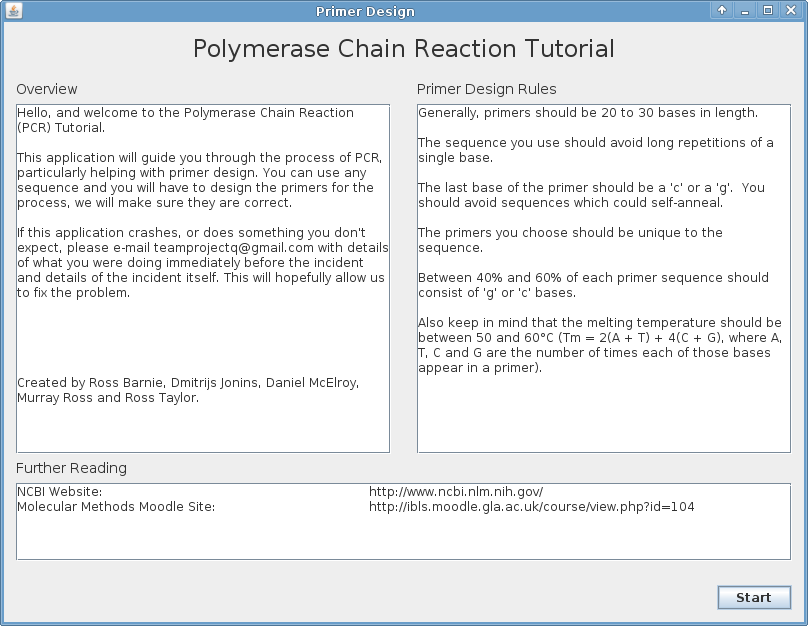
\includegraphics[width=0.5\textwidth]{./images/demoBuild/splash.png}
    \caption{
      \label{fig:demoBuild:splash}
      Demo Build, Overview Panel 
    }
  \end{center}
\end{figure}

\paragraph{Sequence Entry}

\begin{figure}[h!]
  \begin{center}
    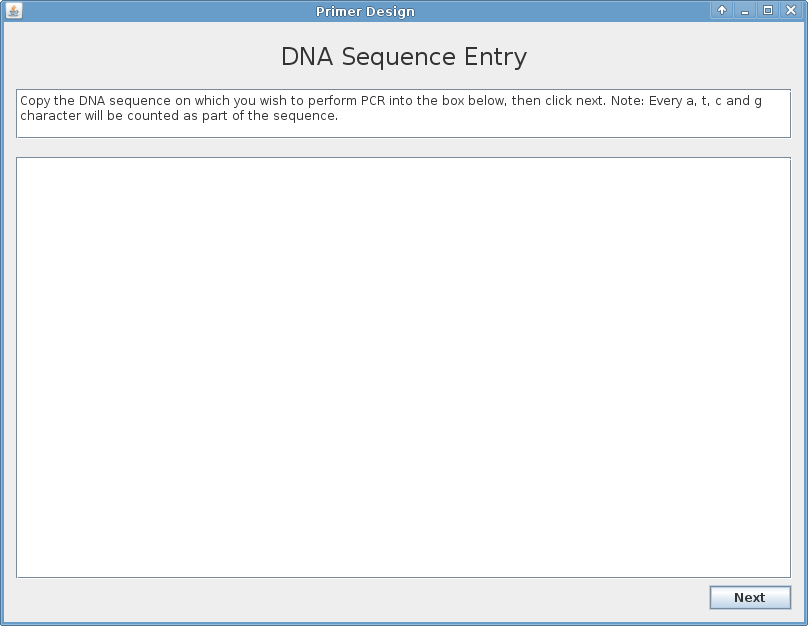
\includegraphics[width=0.5\textwidth]{./images/demoBuild/sequenceEntry.png}
    \caption{
      \label{fig:demoBuild:sequenceEntry}
      Demo Build, sequence entry panel 
    }
  \end{center}
\end{figure}

Figure \ref{fig:demoBuild:sequenceEntry} shows the next panel,
referred to by the team as the ``sequence entry'' panel.
While based on the design in figure *REFERENCE INITIAL UI DESIGN* it
has been altered slightly to maximise the amount of space to be used
for entering in the sequence, as this is the primary purpose of this
panel.

It was expected of the user to go to the National Center for
Biotechnology Information (NCBI) website and obtain a DNA sequence by
copying it to their clipboard and then pasting this into the sequence
entry panel and this was explained in the accompanying user guide
(appendix *USER GUIDE APPENDIX*).
Although this relied heavily on the users' ability to use keyboard
shortcuts, it was assumed that all students at university level would
at least have an awareness of these shortcuts.
We also assumed that once students were told of these shortcuts, as
they were in the user guide, that they would be comfortable using
them.

%---------------------------------------------------------------------

\paragraph{Area Selection}

\begin{figure}[h]
  \begin{center}
    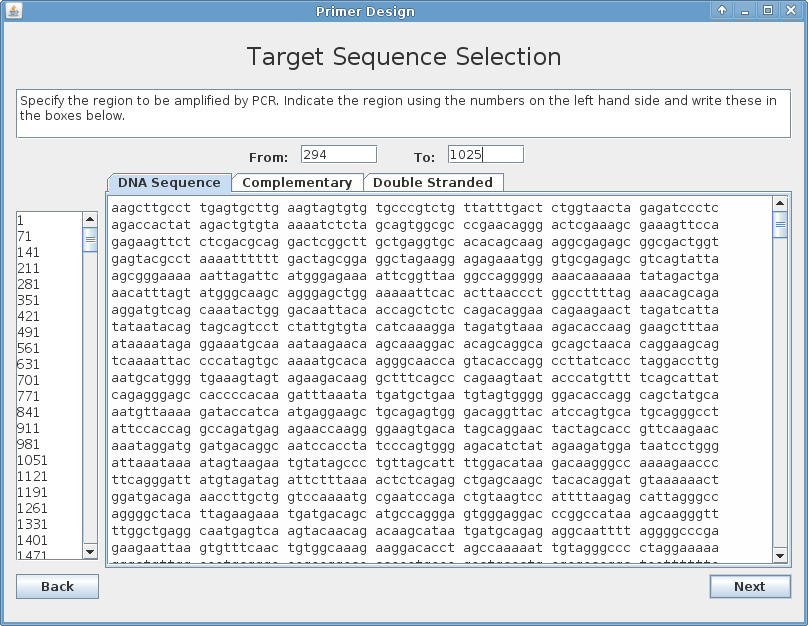
\includegraphics[width=0.5\textwidth]{./images/demoBuild/areaSelection.png}
    \caption{
      \label{fig:demoBuild:areaSelection}
      Demo Build, Area Selection Panel
    }
  \end{center}
\end{figure}

Following the Sequence Entry panel is the ``Area Selection'' panel,
seen in figure \ref{fig:demoBuild:areaSelection}, which requires the
user to specify the ``target'' sequence, ie the desired output
sequence of the PCR process.
This is accomplished by the user entering the start of the sequence
that they want and the end of the sequence they want, both by the
index of that base in the sequence, into the ``From'' and ``To''
fields at the bottom of the panel.

This would, ideally, be helped by the text pane at the left of the
screen which shows the base number of the first base on its line.
Unfortunately, for an unknown reason, the text panes became misaligned
when viewed from any platform other than the one we were using for
development (the level 3 Computing Science Laboratory computers
running Scientific Linux) and this misalignment can be seen in figure
\ref{fig:demoBuild:areaSelection}.

An addition made to the design discussed in *REFERENCE DESIGN* is the
tabs above the main text area, which allow the user to switch between
the sequence they entered, and its complementary equivalent, generated
by the program.
It was a suggestion by the clients to have this feature as it would
greatly increase the speed at which the user could design the reverse
primer.
Without the complementary tab, not only would the user have to
manually convert the primer to its complementary equivalent, but also
reverse its order, which neither the team or the clients felt was a
useful way for students to spend their time. 

%---------------------------------------------------------------------

\paragraph{Primer Design}

Following the Area Selection panel is the ``Primer Design'' panel,
shown in figure \ref{fig:demoBuild:primerDesign}, which allows the
user to enter forward and reverse primers.

\begin{figure}[h]
  \begin{center}
    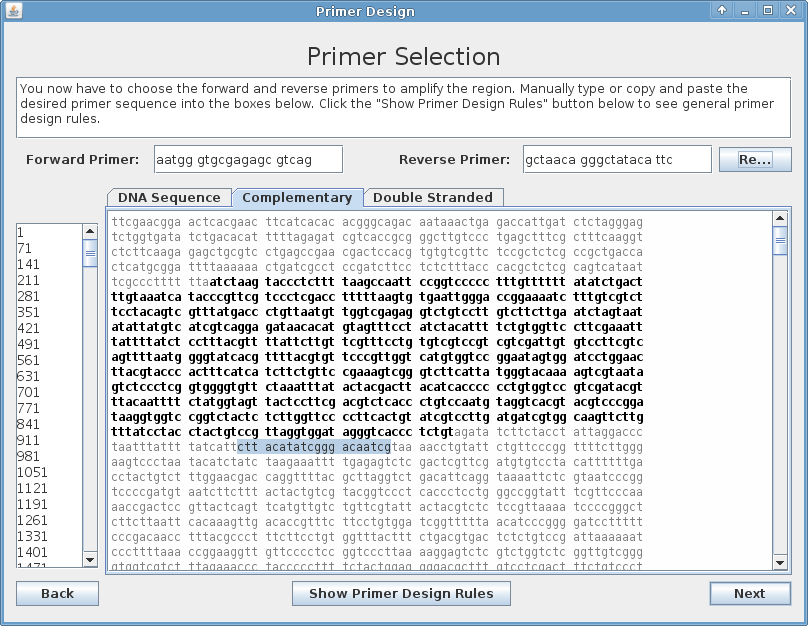
\includegraphics[width=0.5\textwidth]{./images/demoBuild/primerDesign.png}
    \caption{
      \label{fig:demoBuild:primerDesign}
      Demo Build, Primer Design Panel
    }
  \end{center}
\end{figure}

One of the design features we had intended to provide was ``dynamic
highlighting'', as referred to by the team, which was going to provide
a highlight around what the user enters into the primer text fields.
This highlighting was unfortunately missing in the demo build due to
time constraints.

However, we had always intended to give feedback to the user should
they break rules of primer design and the demo build version of this
can be seen in figure \ref{fig:demoBuild:primerFeedback}.

Again based on the design *REFERENCE*, this dialogue window shows the
user any rules which they have broken, and which primer the feedback
is referring to.
In terms of user-friendliness and design it could have used a lot of
improvement however this was a feature still in early development.

\begin{figure}[h]
  \begin{center}
    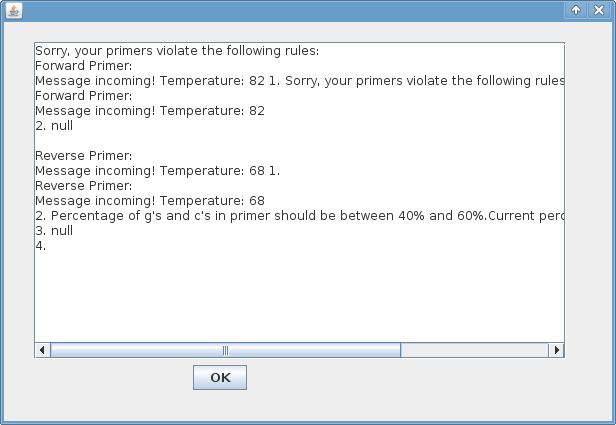
\includegraphics[width=0.5\textwidth]{./images/demoBuild/primerFeedback.png}
    \caption{
      \label{fig:demoBuild:primerFeedback}
      Demo Build, Feedback on User-entered Primer
    }
  \end{center}
\end{figure}

Again, due to time constraints this was not as fully featured as we
had hoped for in the demonstration, however it did display enough
information to give an idea to our clients of what the feedback might
look like in the future (see further discussion in section *REFERENCE
DEMO FEEDBACK SECTION*)

\paragraph{Melting Temperature}

After designing a primer, the user is presented with the ``Melting
Temperature'' panel as seen in figure \ref{fig:demoBuild:meltingTemp}
for the user to evaluate their primers.

In the case of the demonstration, this panel was blocked from the user
unless they had a correct primer.

\begin{figure}[h]
  \begin{center}
    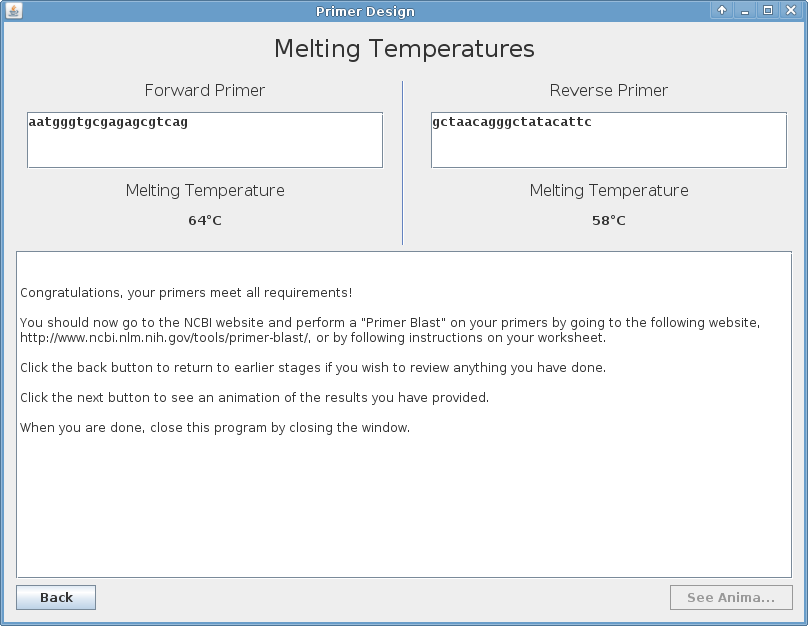
\includegraphics[width=0.5\textwidth]{./images/demoBuild/meltingTemp.png}
    \caption{
      \label{fig:demoBuild:meltingTemp}
      Demo Build, Melting Temperatures of User's Primers.
    }
  \end{center}
\end{figure}

In terms of design, the initial design proved to be near-impossible to
reproduce in Swing and make it look professional and after several
iterations became what it is.
The emphasis on the primers and the melting temperatures in bold means
that the user can easily see their primers and the associated melting
temperatures, while the separator down the center visually separates
the forward from the reverse primer.

Unfortunately the animation was not available in time for the
demonstration and although the button for it was included in this
panel it was disabled.

